%%%%%%%%%%%%%%%%%%%%%%%%%%%%%%%%%%%%%%%%%%%%%%%%%%%%%%%%%%%%%%%%%%%%%%
% Problem statement
\begin{statement}[
  problempoints=20,
  timelimit=1 sekunda,
  memorylimit=512 MiB,
]{Koeficijent}

\setlength\intextsep{-0.1cm}
\begin{wrapfigure}[5]{r}{0.2\textwidth}
\centering
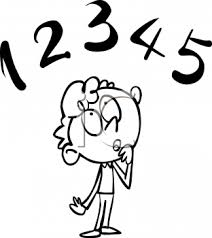
\includegraphics[width=0.2\textwidth]{img/plenki.jpeg}
\end{wrapfigure}

Andrej voli brojeve rastavljati na zbrojeve. Tako kada mu netko kaže broj $6$,
on kaže $3+1+2$. Preciznije, za zadani prirodan broj $N$, Andrej kaže izraz
oblika $A_1+A_2+\dots+A_x$, pri čemu su $A_i$ prirodni brojevi takvi da je
$A_1+A_2+\dots+A_x=N$. U izrazu trebaju biti najmanje dva pribrojnika.

Napišite program koji za zadani prirodan broj $N$ ispisuje bilo koji izraz koji
zadovoljava Andrejeve uvjete rastavljanja.


%%%%%%%%%%%%%%%%%%%%%%%%%%%%%%%%%%%%%%%%%%%%%%%%%%%%%%%%%%%%%%%%%%%%%%
% Input
\subsection*{Ulazni podaci}
U prvom je retku prirodan broj $N$ $(1 \le N \le 100)$ iz teksta zadatka.

%%%%%%%%%%%%%%%%%%%%%%%%%%%%%%%%%%%%%%%%%%%%%%%%%%%%%%%%%%%%%%%%%%%%%%
% Output
\subsection*{Izlazni podaci}
U jedini redak ispišite bilo koji traženi izraz u zadanom obliku. Razmaci u
ispisu nisu dozvoljeni.

%%%%%%%%%%%%%%%%%%%%%%%%%%%%%%%%%%%%%%%%%%%%%%%%%%%%%%%%%%%%%%%%%%%%%%
% Scoring
 %\subsection*{Bodovanje}

%%%%%%%%%%%%%%%%%%%%%%%%%%%%%%%%%%%%%%%%%%%%%%%%%%%%%%%%%%%%%%%%%%%%%%
% Examples
\subsection*{Probni primjeri}
\begin{tabularx}{\textwidth}{X'X'X}
\sampleinputs{test/koeficijent.dummy.in.1}{test/koeficijent.dummy.out.1} &
\sampleinputs{test/koeficijent.dummy.in.2}{test/koeficijent.dummy.out.2} &
\sampleinputs{test/koeficijent.dummy.in.3}{test/koeficijent.dummy.out.3}
\end{tabularx}

\textbf{Pojašnjenje probnih primjera:}
Broj $6$ moguće je na više načina zapisati kao zbroj pribrojnika. U probnim su
primjerima pokazana neka tri načina.

%%%%%%%%%%%%%%%%%%%%%%%%%%%%%%%%%%%%%%%%%%%%%%%%%%%%%%%%%%%%%%%%%%%%%%
% We're done
\end{statement}

%%% Local Variables:
%%% mode: latex
%%% mode: flyspell
%%% ispell-local-dictionary: "croatian"
%%% TeX-master: "../hio.tex"
%%% End:
